Questo capitolo illustra nel dettaglio la realizzazione del \emph{backend} della piattaforma CAMUS. Il capitolo si apre con l'esposizione dei descrittori dell'\emph{albero del contesto} e dei \emph{servizi}. Verrà fornita un'analisi degli attributi che li caratterizzano, con l'ausilio di esempi per chiarire meglio i concetti. In seguito verrà mostrato il diagramma \emph{Entità-Relazione} del database e lo schema logico che ne consegue. Verrà esposto in seguito il diagramma delle classi del \emph{backend} e vengono analizzati i dettagli implementativi dei singoli componenti. Una sezione verrà dedicata all'\emph{endpoint} GraphQL, che permette alle applicazioni esterne di eseguire le attività messe a disposizione dal \emph{backend}. Il capitolo termina con la documentazione relativa alla configurazione del sistema, che permette la definizione di alcuni parametri utilizzati in fase di esecuzione per modificarne il comportamento. Una configurazione può essere definita tramite variabili d'ambiente o file di configurazione. Verranno descritte entrambe le possibilità.

\section{Descrittore dell'albero di contesto\label{sec:descrittore-albero-contesto}}

Nella Sezione \ref{sec:context-dimension-model} è stato esposto il modello teorico del \emph{Context Dimension Tree} mentre in questa sezione si vuole mettere in risalto come l'albero di contesto viene descritto nel sistema. Sono state effettuate diverse semplificazioni per agevolare la memorizzazione e il recupero delle informazioni dai vari nodi che compongono l'albero. Nelle seguenti sottosezioni vengono analizzati nel dettaglio i singoli oggetti che formano un albero di contesto.

\subsection{Radice\label{sec:radice-cdt}}

Questo oggetto rappresenta la radice di un albero di contesto. \upe composto dai seguenti parametri:

\begin{itemize}
	\item \textbf{User Id}
	L'elenco degli identificativi degli utenti ai quali questo albero è associato. Viene lasciata la possibilità di definire più utenti perché uno stesso albero può essere valido per più utenti con un profilo simile
	\item \textbf{Context}
	Contiene i \emph{nodi} che compongono l'albero. Per una descrizione approfondita si fa riferimento alla Sezione \ref{sec:nodo-cdt}
	\item \textbf{Default Values}
	Vengono elencati tutti i valori che l'\emph{esperto di settore} ha specificato siano sempre validi per gli utenti ai quali questo albero viene associato. \upe composto dal nome della \emph{dimensione} e dal relativo \emph{valore} che assume
\end{itemize}

Viene inoltre definito un \emph{CDT Globale}, utilizzato come base per la creazione di quelli specifici per ogni utente. Questo albero ha la particolarità che non è associato a nessun utente.

\subsection{Nodi\label{sec:nodo-cdt}}

Questo oggetto rappresenta un nodo dell'albero. In particolare vengono rappresentati solamente i nodi di tipo \emph{dimensione} tramite oggetti dedicati, mentre i nodi \emph{contesto} e \emph{parametro} vengono rappresentati come sottocomponenti. Ogni nodo possiede i seguenti attributi:

\begin{itemize}
	\item \textbf{Name}
	Il nome del nodo dimensione
	\item \textbf{For}
	Descrive la tipologia di nodo, utilizzata per assegnare un peso utile nella fase di \emph{selezione delle operazioni} e per attribuire un valore ai parametri nella fase di \emph{invocazione dei servizi}. I valori ammessi sono \emph{filter}, \emph{parameter} o \emph{ranking}. Vengono inoltre ammesse le combinazioni \emph{filter}|\emph{parameter} e \emph{ranking}|\emph{parameter}: un nodo può essere solamente di tipo \emph{filter} o \emph{ranking}, al fine dell'assegnamento dei pesi, mentre può essere anche di tipo \emph{parameter}, in quanto indica che verrà utilizzato anche nella fase di composizione delle \emph{query}. Se viene definito il tipo \emph{parameter} devono essere assegnati diversi \emph{parametri}, per specificarne le caratteristiche
	\item \textbf{Values}
	Elenca i possibili valori che può assumere il nodo. Questo elenco corrisponde ai nodi di tipo \emph{contesto} del modello del CDT
	\item \textbf{Parameters}
	L'elenco dei parametri associati al nodo. Per ulteriori dettagli su questo oggetto si fa riferimento alla Sezione \ref{sec:parametro-cdt}
	\item \textbf{Parents}
	Contiene l'elenco di tutti i nodi dimensione dai quali discende il nodo corrente. Viene utilizzato per effettuare l'unione delle sottodimensioni di un nodo
\end{itemize}

Nel Listato \ref{lst:esempio-nodo-cdt} viene mostrato un esempio di nodo.

\begin{listing}[h]
	\inputminted{json}{5-implementazione-backend/Codice/esempio_nodo_cdt.json}
	\caption{Esempio di nodo del CDT}
	\label{lst:esempio-nodo-cdt}
\end{listing}

\subsection{Parametri dei nodi\label{sec:parametro-cdt}}

Questo oggetto definisce i parametri che sono associati a un nodo dimensione. Corrisponde ai nodi di tipo \emph{parametro} del modello del CDT. I parametri vengono utilizzati per permettere all'utente di specificare dei valori di sua scelta (es.: località). \upe composto dai seguenti campi:

\begin{itemize}
	\item \textbf{Name}
	Il nome del parametro
	\item \textbf{Type}
	Il/I formato/i del dato che vengono accettati
	\item \textbf{Fields}
	Questo elenco permette di definire dei campi che vanno ulteriormente a specificare il parametro. Un esempio viene dato dal parametro \virgolette{Luogo}, che può essere specializzato nei campi \virgolette{Latitudine} e \virgolette{Longitudine}
\end{itemize}

Nel Listato \ref{lst:esempio-parametro-cdt} viene mostrato un esempio di parametro.

\clearpage

\begin{listing}[ht]
	\inputminted{json}{5-implementazione-backend/Codice/esempio_parametro_cdt.json}
	\caption{Esempio di parametro associato a un nodo}
	\label{lst:esempio-parametro-cdt}
\end{listing}

\section{Descrittore dei servizi\label{sec:descrittore-servizi}}

Affinché il sistema possa effettuare le richieste è necessario che sia presente un formato per descrivere le caratteristiche di ogni servizio (es.: l'indirizzo verso il quale effettuare la richiesta, i parametri da inserire, ecc.). Per questo motivo è stato introdotto l'utilizzo di un \emph{descrittore dei servizi} in grado di specificare tutte le possibili configurazioni che i servizi possono richiedere. I \emph{descrittori} non sono altro che configurazioni dei servizi espressi tramite file JSON. Di seguito verranno analizzati nel dettaglio tutti i campi che compongono il descrittore. \upe stata separata la definizione delle informazioni generali del servizio dalle informazioni di dettaglio delle operazioni che espone. Il risultato sono due oggetti, uno di \virgolette{descrizione generale del servizio} e un \virgolette{descrittore delle operazioni}. Nelle seguenti sezioni verranno analizzati gli attributi di entrambi gli oggetti.

\subsection{Descrizione generale del servizio\label{sec:oggetto-principale-servizi}}

\upe il punto di partenza per la descrizione di un servizio. Comprende i seguenti campi:

\begin{itemize}
	\item \textbf{Name}
	Il nome del servizio
	\item \textbf{Description}
	Fornisce una descrizione delle funzionalità del servizio
	\item \textbf{Protocol}
	Definisce la tipologia con la quale accedere al servizio. Può assumere i valori \virgolette{rest}, \virgolette{query} o \virgolette{custom}, per specificare rispettivamente che il servizio viene invocato secondo il protocollo REST, viene composta una query con parametri o è necessario invocare un metodo particolare per l'accesso
	\item \textbf{Base Path}
	Rappresenta l'indirizzo di base del servizio. A partire da questo indirizzo verrà composto quello completo aggiungendo in coda i percorsi specifici delle \emph{operazioni} richieste. Non deve essere inserito al termine nessuno \emph{slash} (\virgolette{/})
\end{itemize}

Nel Listato \ref{lst:esempio-descrittore-servizio} viene mostrato un esempio di oggetto principale del servizio.

\begin{listing}[h]
	\inputminted{json}{5-implementazione-backend/Codice/esempio_descrittore_servizio.json}
	\caption{Esempio di servizio}
	\label{lst:esempio-descrittore-servizio}
\end{listing}

\subsection{Descrittore delle operazioni\label{sec:descrittore-operazioni}}

Rappresenta le operazioni che sono messe a disposizione dal servizio. Un'o\-pe\-ra\-zio\-ne viene descritta dai seguenti campi:

\begin{itemize}
	\item \textbf{Service}
	Contiene il riferimento al \emph{descrittore generale del servizio} associato all'operazione. Un'operazione può essere collegata esclusivamente ad un solo servizio
	\item \textbf{Name}
	Il nome dell'operazione
	\item \textbf{Type}
	Rappresenta la tipologia dell'operazione. Un'operazione può essere \emph{primaria} o di \emph{supporto}. Questa distinzione viene utilizzata principalmente per permettere la catalogazione delle operazioni da mostrare nelle \emph{web app}
	\item \textbf{Description}
	La descrizione dell'attività svolta dall'operazione
	\item \textbf{Path}
	Il percorso specifico per richiamare l'operazione. Questo valore viene aggiunto al \emph{Base Path} del servizio. Deve essere sempre preceduto da una \emph{slash} (\virgolette{/})
	\item \textbf{Protocol}
	Permette di ridefinire il protocollo utilizzato esclusivamente per l'operazione corrente. \upe utile nei casi in cui un'operazione, per una qualsiasi ragione, utilizzi un paradigma di composizione della \emph{query} diverso da quello specificato dal servizio. Per esempio, viene utilizzato per mappare gli \virgolette{intent} su diversi sistemi operativi dei dispositivi, che hanno diverse regole di composizione. Oltre alle tipologie definite per i \emph{servizi} supporta anche il protocollo \virgolette{android}
	\item \textbf{Store Link}
	Utilizzato esclusivamente per i servizi di supporto, permette di definire il \emph{link} nello \emph{store} di riferimento per scaricare l'\emph{app} necessaria a utilizzare l'\emph{intent} associato
	\item \textbf{Bridge Name}
	Questo campo è opzionale, definisce il nome del \emph{bridge} con la logica necessaria per invocare il servizio. \upe obbligatorio il suo utilizzo quando per il servizio viene utilizzato il protocollo \emph{custom}
	\item \textbf{Parameters}
	Definisce l'elenco dei parametri accettati in ingresso dall'o\-pe\-ra\-zio\-ne. Per ulteriori dettagli su questo oggetto si fa riferimento alla Sezione \ref{sec:descrittore-parametri}
	\item \textbf{Headers}
	Permette di specificare gli attributi da aggiungere all'\emph{header} della richiesta. Vengono utilizzati i campi \virgolette{name} per specificare il nome dell'at\-tri\-bu\-to e \virgolette{value} per specificarne il valore
	\item \textbf{Response Mapping}
	Serve per definire le regole di associazione per mappare la risposta del servizio coi termini semantici utilizzati dal sistema. Maggiori dettagli su questo oggetto vengono discussi nella Sezione \ref{sec:descrittore-risposta}
	\item \textbf{Pagination}
	Serve a raccogliere gli attributi necessari per gestire la paginazione specifica di ogni servizio. Sono supportati meccanismi di paginazioni basati sul \emph{numero di pagina} o su \emph{token}. Questo oggetto viene analizzato nel dettaglio nella Sezione \ref{sec:descrittore-paginazione}
\end{itemize}

Nel Listato \ref{lst:esempio-descrittore-operazione} viene mostrato un esempio di operazione. Nel campo \virgolette{service} viene inserito il nome del servizio associato al posto del suo identificativo per maggiore chiarezza.

\begin{listing}[h]
	\inputminted{json}{5-implementazione-backend/Codice/esempio_descrittore_operazione.json}
	\caption{Esempio di operazione}
	\label{lst:esempio-descrittore-operazione}
\end{listing}

\subsection{Parametri delle operazioni\label{sec:descrittore-parametri}}

Quest'oggetto definisce i parametri in ingresso di un'operazione. I parametri generalmente sono composti da due campi: uno ne definisce il \emph{nome} e l'altro il rispettivo \emph{valore}. In alcuni casi vengono accettati più valori, quindi il descrittore deve dunque essere in grado di gestire questa situazione. Un ulteriore compito affidato a questo oggetto è quello di acquisire il valore di un determinato parametro dal \emph{contesto}. Viene inoltre fornito un semplice sistema di traduzione dei dati acquisiti dal contesto, per permettere le trasformazioni verso un valore idoneo per l'operazione corrente. Infine, soprattutto per le operazioni di \emph{supporto}, viene permessa un'associazione del parametro verso uno o più \emph{termini semantici}, per permettere alla \emph{mobile app} di conoscere l'attributo dove andare a recuperare il valore concreto a \emph{runtime}. Nello specifico, l'oggetto è così composto:

\begin{itemize}
	\item \textbf{Name}
	Il nome del parametro. Questo campo è \emph{obbligatorio}, in quanto definisce il nome che verrà utilizzato per comporre la \emph{query} per richiedere i dati
	\item \textbf{Description}
	La descrizione della tipologia del parametro
	\item \textbf{Required}
	Specifica se il parametro corrente è obbligatorio o meno in una richiesta. Non definire questo attributo equivale ad assegnargli valore \emph{false}
	\item \textbf{Type}
	Definisce il \emph{tipo} di dato che l'operazione si aspetta di ricevere. Le principali tipologie di dato che vengono inviate verso i servizi sono \emph{stringhe}, \emph{numeri} o \emph{date}
	\item \textbf{Default}
	Indica un valore predefinito per il parametro. Questo campo è particolarmente utile per la \emph{web app} relativa al \emph{Visual Mapping}, in quanto permette di ricevere degli esempi di risposta dei servizi da mostrare all'utente
	\item \textbf{Collection Format}
	Questo campo definisce il \emph{separatore} da utilizzare nel caso siano presenti più valori per il parametro. Sono accettati i seguenti quattro separatori: \emph{i)} \virgolette{csv}, \emph{comma separated values}; \emph{ii)} \virgolette{ssv}, \emph{space separated values}; \emph{iii)} \virgolette{tsv}, \emph{tab separated values}; \emph{iv)} \virgolette{pipes}. Se non specificato viene utilizzato il tipo \emph{csv}
	\item \textbf{Mapping CDT}
	Definisce uno o più nodi dell'albero di contesto dove andare ad acquisire il valore ricevuto dalla \emph{mobile app}. Nel caso vengano associati più di un nodo viene seguito l'ordine di definizione nella fase di composizione della \emph{query}
	\item \textbf{Mapping Term}
	Definisce uno o più termini semantici da associare al parametro. Questi termini vengono utilizzati a \emph{runtime} per andare ad acquisire il valore del parametro dalle risposte ricevute dai servizi primari
	\item \textbf{Translate}
	Permette delle semplici trasformazioni dei valori acquisiti dall'al\-be\-ro di contesto per renderli conformi a quelli accettati dal servizio. \upe formato dai campi \virgolette{from} e \virgolette{to}, che specificano rispettivamente il valore di \emph{origine} e quello \emph{tradotto}. Vengono definite tante traduzioni quanti sono i valori che può assumere il rispettivo nodo del CDT
\end{itemize}

Nel Listato \ref{lst:esempio-descrittore-parametro} viene mostrato un esempio di parametro di un'operazione.

\begin{listing}[h]
	\inputminted{json}{5-implementazione-backend/Codice/esempio_descrittore_parametro.json}
	\caption{Esempio di parametro di un'operazione}
	\label{lst:esempio-descrittore-parametro}
\end{listing}

\subsection{Formato della risposta\label{sec:descrittore-risposta}}

In quest'oggetto sono definite le regole con le quali vengono trasformate le risposte ricevute dal servizio nel formato interno CAMUS, dove ogni attributo viene associato a un rispetto \emph{termine semantico} che ne definisce il contenuto. In particolare, vengono utilizzati i seguenti campi:

\begin{itemize}
	\item \textbf{List}
	Definisce l'attributo che contiene l'elenco dei risultati. \upe utile nei casi in cui la risposta, oltre ai risultati, contiene al suo interno anche dei metadati relativi l'interrogazione. Se non specificato si assume che l'elenco dei risultati si trovi nella radice della risposta
	\item \textbf{Items}
	Permette di mappare i vari campi che compongono ogni oggetto dei risultati. In particolare vengono definiti il \virgolette{percorso} dal quale recuperare il valore e il \virgolette{termine semantico} da associare. I campi senza un'associazione saranno ignorati dal processo di trasformazione e le relative informazioni andranno perdute. \upe necessario dunque effettuare l'operazione di \emph{mapping} delle risposte con attenzione, in modo da non trascurare informazioni importanti
	\item \textbf{Functions}
	Viene permesso l'utilizzo di funzioni specifiche per trasformare i valori. Questa funzione riceve in ingresso il parametro \virgolette{value}, che rappresenta il valore corrente del campo, e deve restituire il nuovo valore che verrà sostituito a quello originale. Oltre alla funzione specifica è necessario definire anche l'\emph{attributo} sul quale eseguire questa trasformazione. L'attributo equivale al \emph{termine semantico} definito nel punto precedente
\end{itemize}

Nel Listato \ref{lst:esempio-formato-risposta} viene mostrato un esempio di formato di risposta.

\begin{listing}[h]
	\inputminted{json}{5-implementazione-backend/Codice/esempio_formato_risposta.json}
	\caption{Esempio di formato di risposta}
	\label{lst:esempio-formato-risposta}
\end{listing}

\subsection{Paginazione\label{sec:descrittore-paginazione}}

In quest'oggetto vengono descritti gli attributi necessari per gestire la paginazione delle risposte. In particolare il sistema è in grado di gestire due tecniche di paginazione, quella basata sul \emph{numero di pagina} e quella che utilizza dei \emph{token} per richiamare le pagine. L'oggetto è composto dai seguenti campi:

\begin{itemize}
	\item \textbf{Attribute Name}
	Specifica il nome del parametro da aggiungere alla \emph{query} per richiamare una specifica pagina
	\item \textbf{Type}
	Definisce il meccanismo di paginazione da utilizzare. Sono ammessi due valori: \virgolette{number}, per la paginazione basata sul numero di pagine, e \virgolette{token}, per quella che sfrutta i \emph{token} per richiamare le pagine successive
	\item \textbf{Token Attribute}
	Serve per definire dove andare a leggere nella risposta il \emph{token} relativo alla pagina successiva
	\item \textbf{Page Count Attribute}
	Definisce l'attributo che fornisce l'informazione del numero di pagine totale che possono essere richieste
\end{itemize}

Nel Listato \ref{lst:esempio-descrittore-paginazione} viene mostrato un esempio di descrittore della paginazione.

\begin{listing}[h]
	\inputminted{json}{5-implementazione-backend/Codice/esempio_descrittore_paginazione.json}
	\caption{Esempio di descrittore della paginazione}
	\label{lst:esempio-descrittore-paginazione}
\end{listing}

\section{Schema del database\label{sec:schema-database}}

\begin{figure}[p]
	\centering
	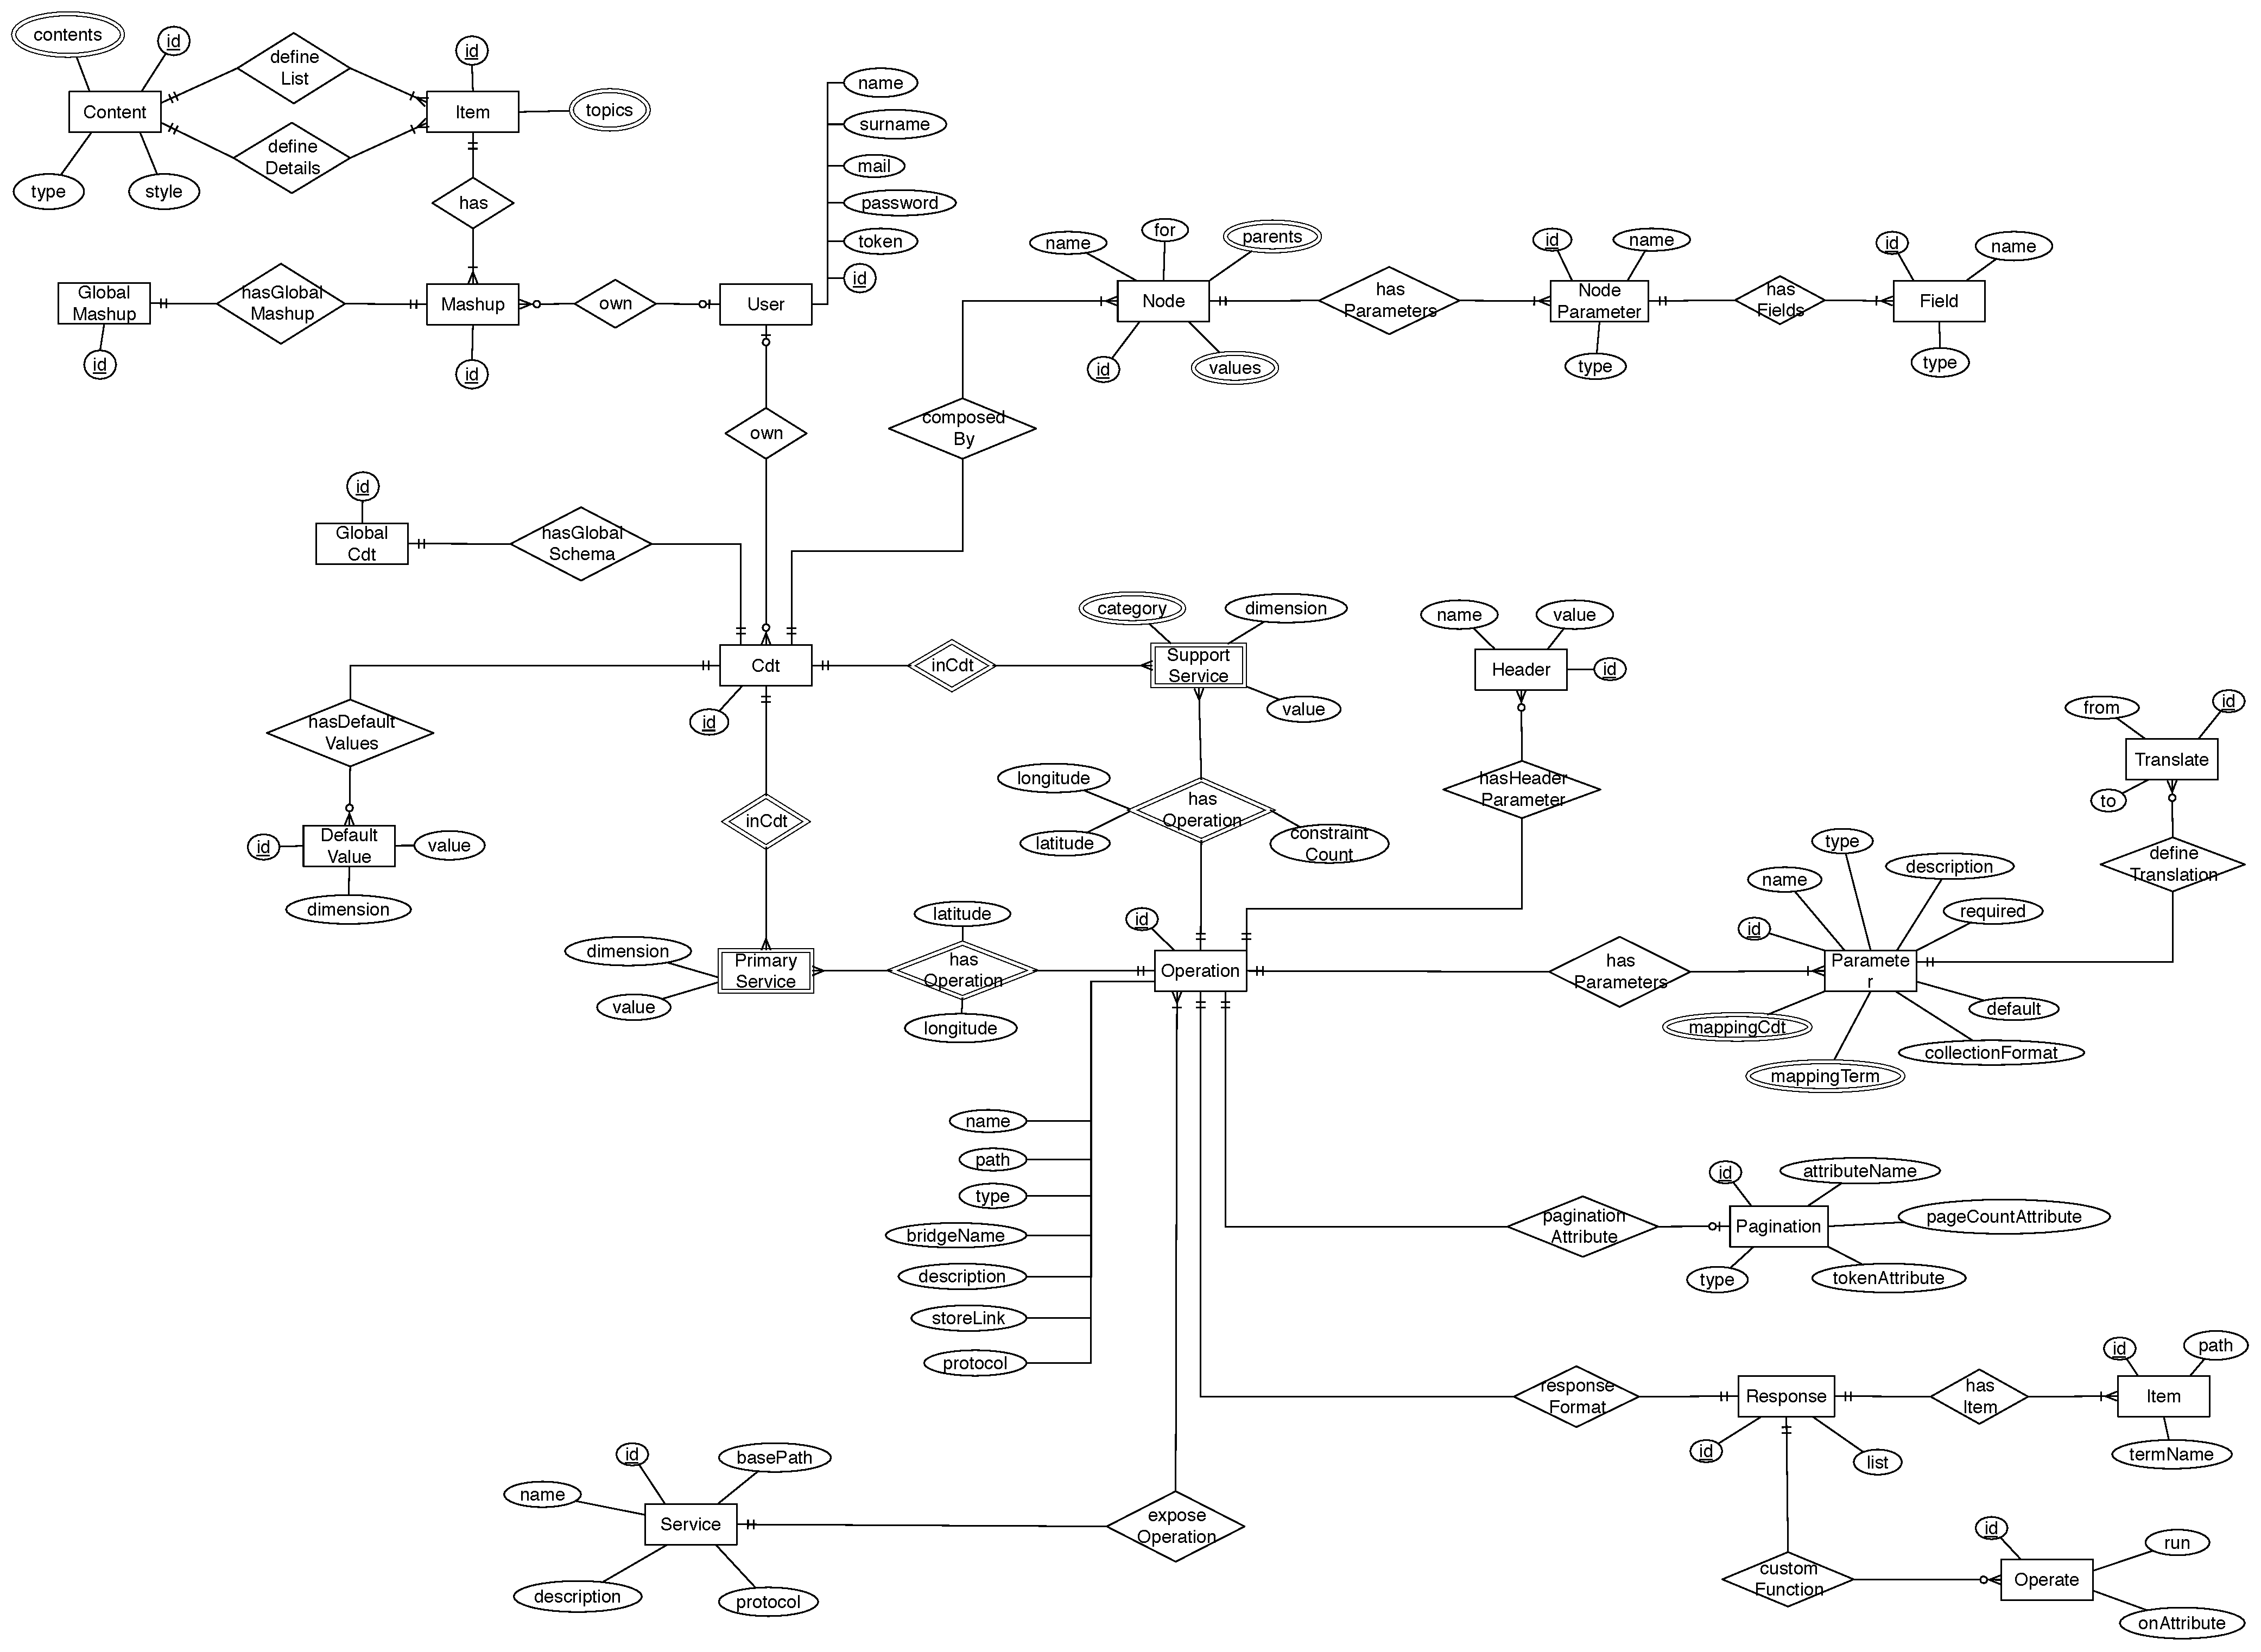
\includegraphics[height=\textwidth, angle=90]{5-implementazione-backend/Immagini/schema_er_db.pdf}
	\caption{Diagramma ER del database}\label{fig:schema-er-db}
\end{figure}

La base di dati viene utilizzata principalmente per garantire la persistenza di cinque elementi: \emph{i)} il descrittore dei servizi, \emph{ii)} l'albero del contesto, \emph{iii)} le associazioni tra operazioni e nodi del CDT, \emph{iv)} le informazioni sugli utenti e \emph{v)} gli schemi di \emph{mashup}. In Figura \ref{fig:schema-er-db} è possibile osservare il modello \emph{Entità-Relazione} utilizzato per la piattaforma CAMUS.

Queste entità permettono al sistema di svolgere le attività principali. Le prime tre entità sono state esposte nelle precedenti sezioni, in quanto si tratta di oggetti complessi che richiedono di una spiegazione dettagliata. Le entità riguardanti i \emph{mashup} vengono associate all'utente per permettere la definizione di schemi personalizzati. Anch'esse necessitano di una descrizione dettagliata, per metterne in risalto le caratteristiche. La loro composizione verrà esposta nella Sezione \ref{sec:struttura-schemi-mashup}.

Una volta definito il modello ER è necessario passare alla realizzazione dello \emph{schema logico} del database, quello che verrà effettivamente utilizzato nell'im\-ple\-men\-ta\-zio\-ne. Non esistendo uno standard per realizzare uno schema di questo tipo per i database non relazionali è stato scelto di utilizzare un \emph{diagramma delle classi} per rappresentare i \emph{documenti} che compongono il database. Ogni classe viene intesa come un documento e i collegamenti evidenziati con una linea continua rappresentano i sottodocumenti. Le linee tratteggiate indicano le referenze tra i vari documenti.

In Figura \ref{fig:schema-logico-db} viene mostrato lo schema logico utilizzato per CAMUS.

\begin{figure}[!t]
	\centering
	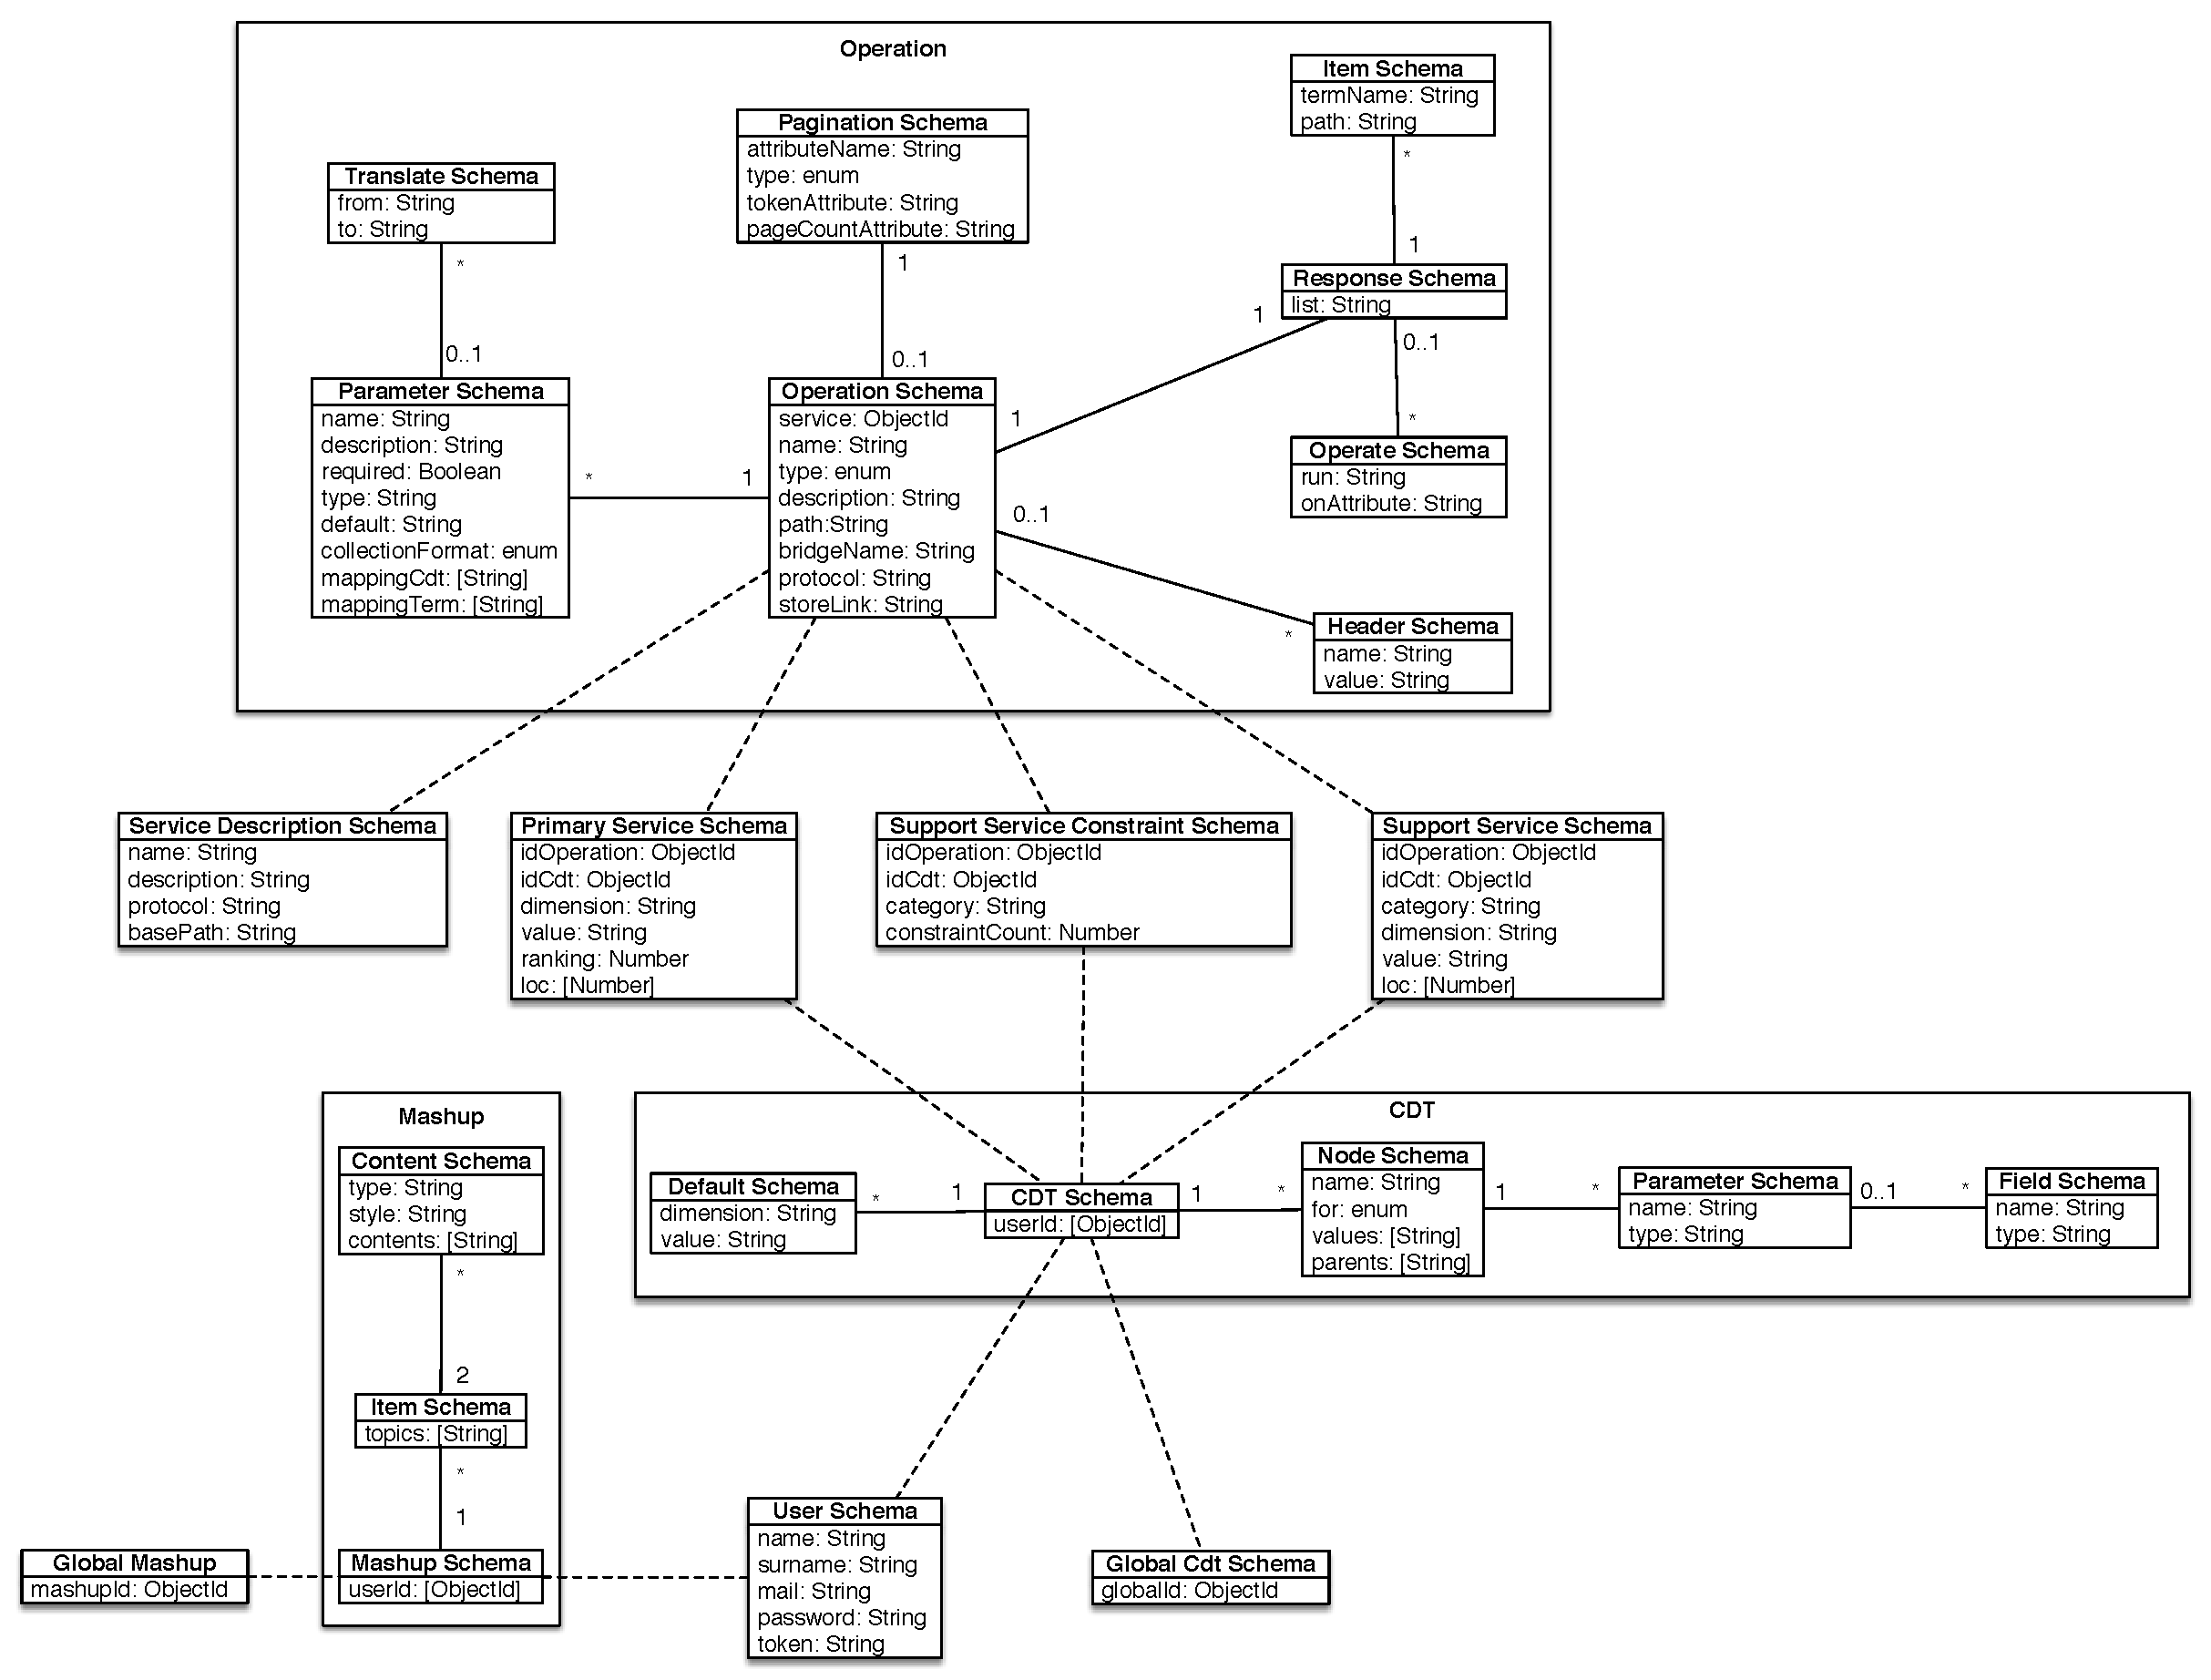
\includegraphics[width=\textwidth]{5-implementazione-backend/Immagini/schema_logico_db.pdf}
	\caption{Schema logico del database}\label{fig:schema-logico-db}
\end{figure}

\section{Componenti\label{sec:componenti-backend}}

\begin{figure}[p]
	\centering
	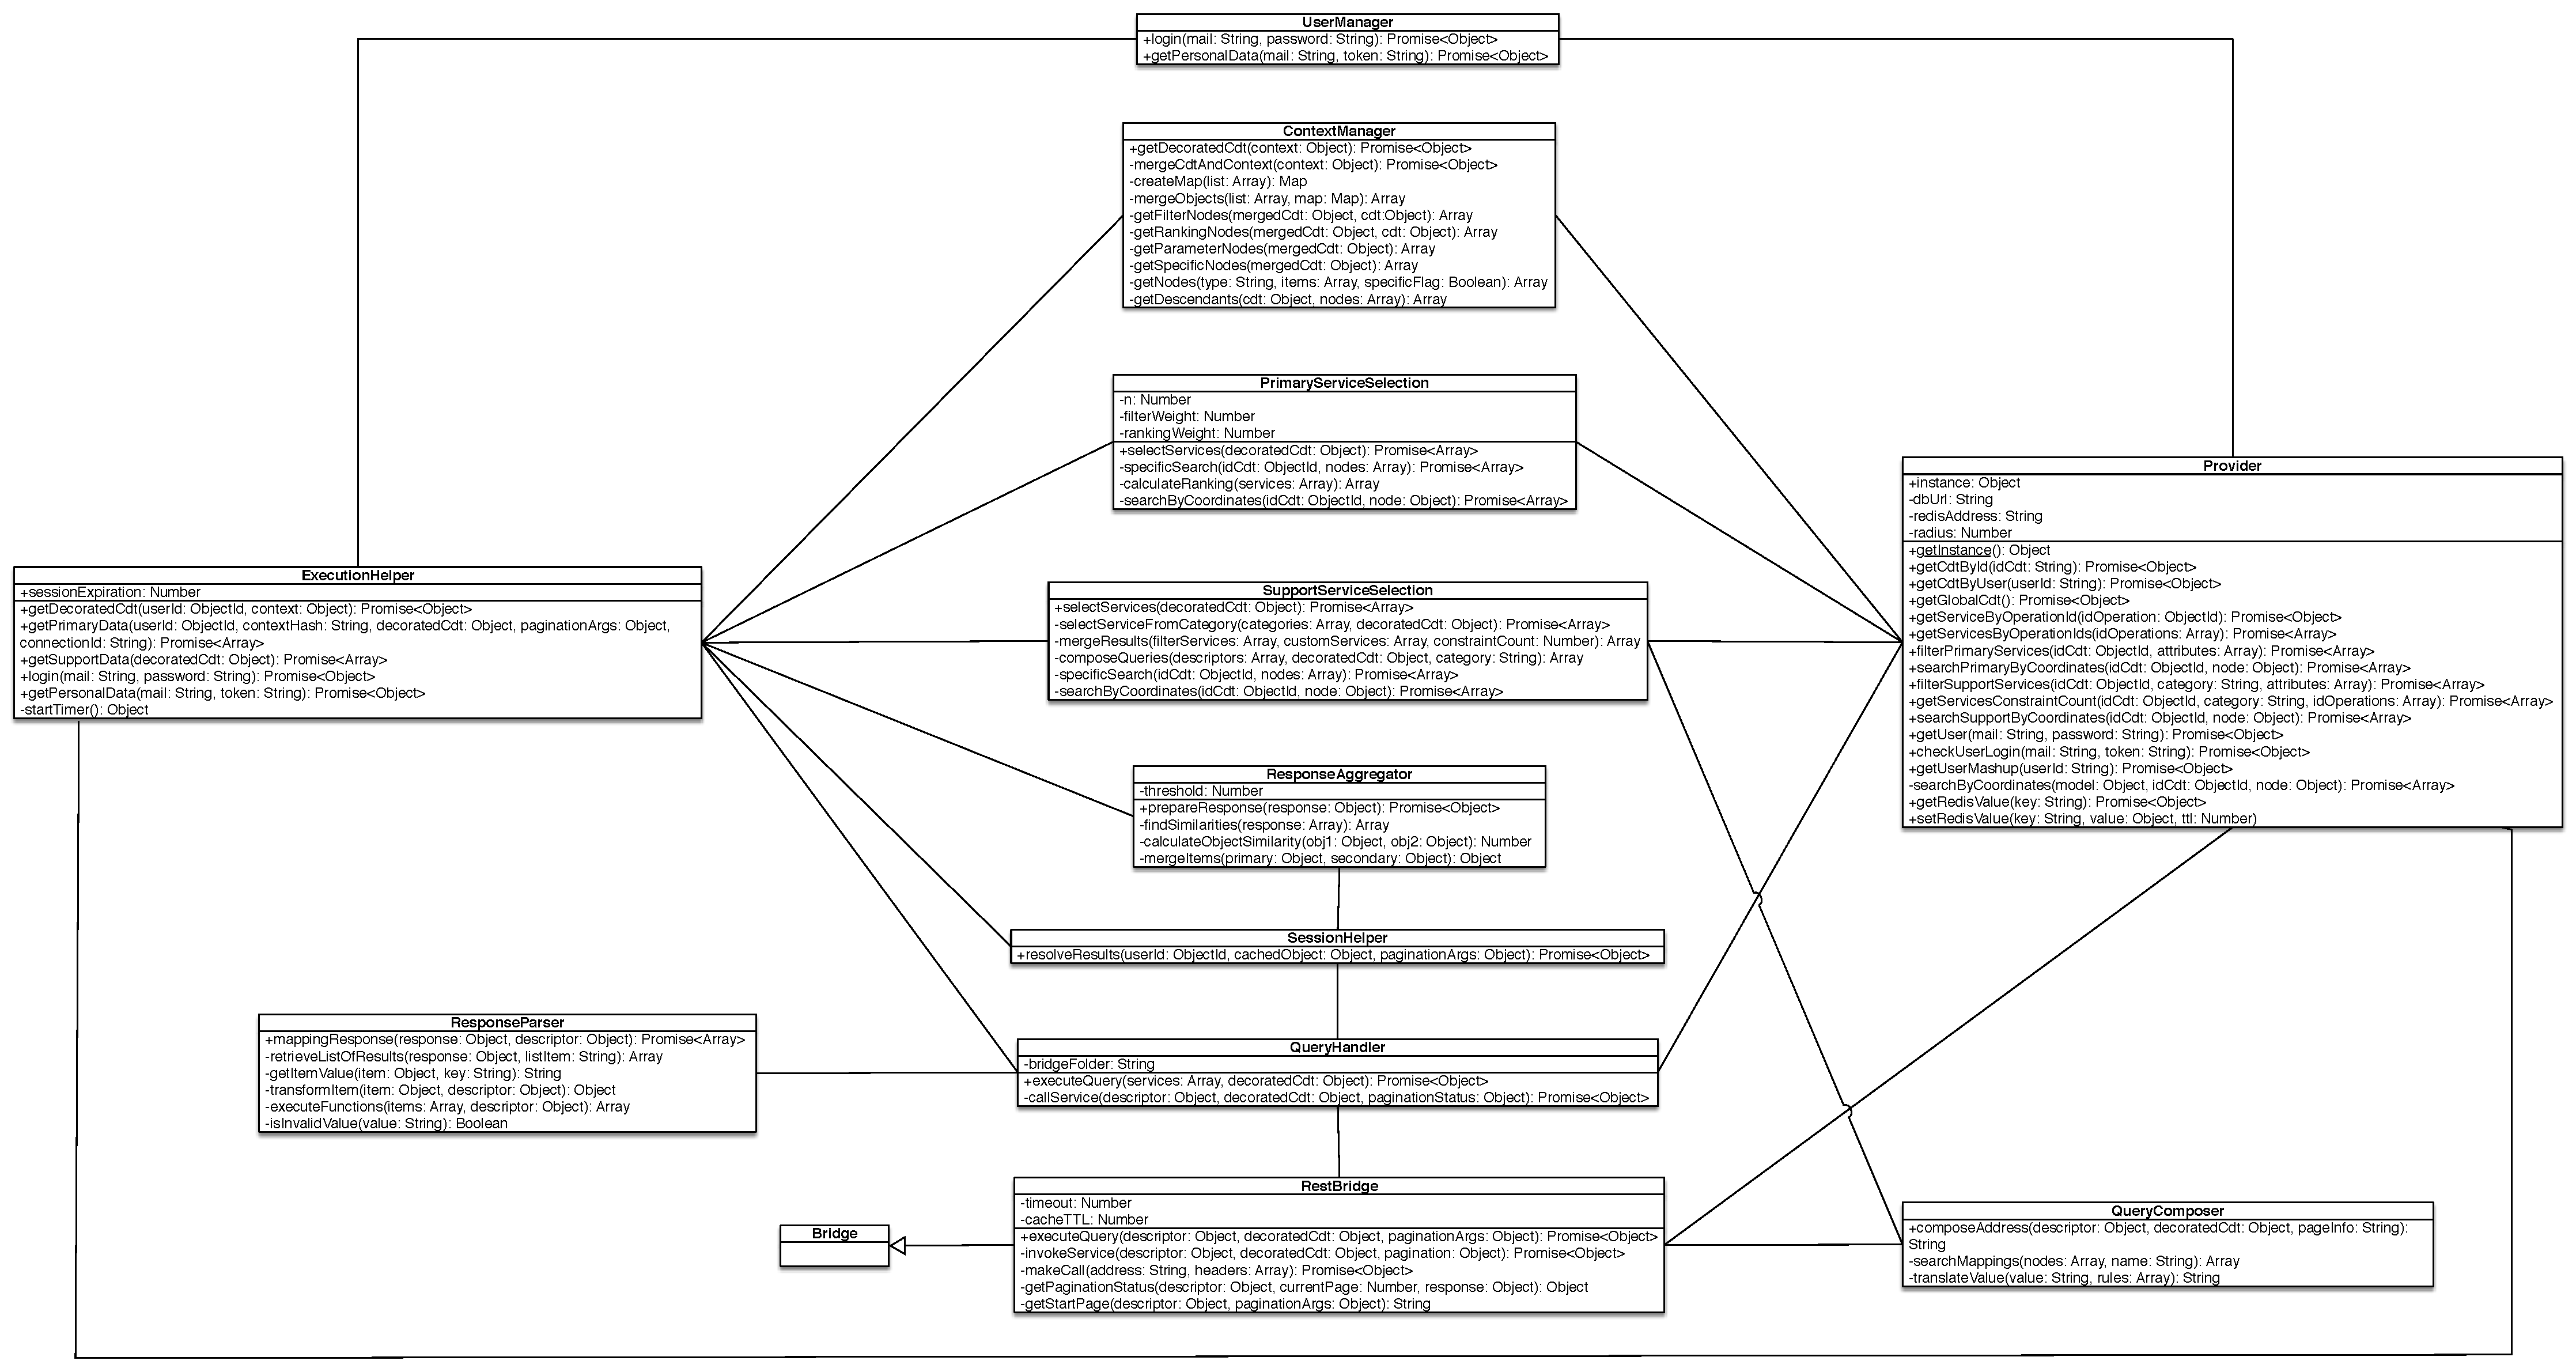
\includegraphics[height=\textwidth, width=\textheight, angle=90]{5-implementazione-backend/Immagini/diagramma_classi_backend.pdf}
	\caption{Diagramma delle classi del backend}\label{fig:class-diagram-backend}
\end{figure}

Come già evidenziato nella Sezione \ref{sec:architettura-backend}, l'architettura del \emph{backend} è composta da diversi \emph{componenti}. Questa soluzione è stata adottata per via dell'elevata flessibilità che garantisce. Ogni componente è specializzato in un compito preciso e il concatenamento di più componenti permette di realizzare funzionalità più complesse per produrre il risultato desiderato. Per svolgere le principali attività vengono dunque create delle \emph{pipeline}, dove il risultato di un componente viene acquisito e ulteriormente elaborato dal successivo.

Altra caratteristica importante è l'assenza di informazioni sullo stato in ogni componente. Una richiesta nasce nel momento in cui l'utente conferma l'attività e muore una volta che viene evasa. La ragione principale di questa scelta risiede nel fatto che sarebbe oneroso lato \emph{backend} gestire tutte le informazioni della moltitudine di utenti che sono connessi al sistema. Inoltre mantenere uno stato limiterebbe la scalabilità del sistema, in quanto se un utente inizia la sessione su di un determinato \emph{server} dovrà continuare sempre su quello, rendendo complicato il bilanciamento dei carichi tra le diverse macchine.

A questo punto è necessaria una importante precisazione: per la gestione della paginazione è necessario l'utilizzo di alcune informazioni sullo stato. Questa affermazione può sembrare un controsenso rispetto a ciò che è stato esposto nel paragrafo precedente. \upe dunque essenziale definire in modo dettagliato cosa si intende per \emph{stato}. La principale differenza consiste nel \emph{dove} vengono salvate le informazioni. Nel paragrafo precedente, ogni volta che si menzionava il concetto di \emph{stato}, si intendevano tutte le informazioni relative l'utente salvate all'\emph{interno} dei componenti, sotto forma di variabile. Questa soluzione può essere un collo di bottiglia non indifferente, in quanto tutte le richieste che nascono in una determinata macchina dovranno essere gestite esclusivamente da essa. Si è adottata quindi una soluzione differente: i \emph{componenti} non mantengono al loro interno alcuna informazione riguardo lo stato, che verrà invece memorizzato e reso disponibile da un servizio esterno. Questa soluzione permette a tutti i componenti che ne hanno esigenza di andare a recuperare le informazioni sullo stato da una sorgente comune, che non limita la scalabilità del sistema. Questo servizio può a sua volta offrire dei sistemi di \emph{clustering} per aumentare le \emph{perfomance} in situazioni di elevato carico.

In CAMUS questa attività viene svolta da \emph{Redis}, che è stato selezionato per l'elevata rapidità nell'evadere le richieste e nella possibilità di associare un periodo di vita alle informazioni che vengono memorizzate. Viene ipotizzato che dopo un intervallo di tempo nel quale l'utente non effettua più interazione sulla sessione, essa può ritenersi estinta e i suoi dati eliminati.

Per gestire le funzionalità del server viene utilizzato il \emph{web framework} \emph{ExpressJS}\footnote{ExpressJS: \url{http://expressjs.com/}}. \emph{ExpressJS} è un \emph{framework} molto leggero, che mette a disposizione le funzionalità base affinché un server sia operativo. Ha la potenzialità di avere un ottimo sistema di \emph{middleware}, che permette di utilizzare altre funzionalità più avanzate.

Per \emph{GraphQL} viene utilizzata l'implementazione specifica per \emph{Javascript} rilasciata da \emph{Facebook}\footnote{GraphQL-js: \url{https://github.com/graphql/graphql-js}} e l'estensione di \emph{Relay}\footnote{Relay-GraphQL: \url{https://github.com/graphql/graphql-relay-js}} per gestire le connessioni. Affinché gli schemi di \emph{GraphQL} possano essere esposti dal server si sfrutta l'apposito \emph{middleware} \emph{Express-GraphQL}\footnote{Express-GraphQL: \url{https://github.com/graphql/express-graphql}}.

\emph{MongoDB} non possiede una struttura dello schema del database definita a priori. Per garantire coerenza coi dati memorizzati si è scelto di utilizzare un \emph{Object Relational Mapping} (ORM)\footnote{Object Relational Mapping: \url{https://it.wikipedia.org/wiki/Object-relational_mapping}}. Un ORM fornisce un livello di astrazione superiore a un driver nativo e permette di specificare come gli oggetti vengono mappati nel database e viceversa, definendo implicitamente uno schema del database. In particolare, per il progetto CAMUS è stato utilizzato un ORM specifico per Node.js di nome \emph{mongoose}\footnote{MongooseJS: \url{http://mongoosejs.com/}}.

Infine, per interfacciare Node.js con l'istanza di Redis in esecuzione viene utilizzato il modulo \emph{ioredis}\footnote{ioredis: \url{https://github.com/luin/ioredis}}.

In Figura \ref{fig:class-diagram-backend} viene mostrato il diagramma delle classi di tutti i componenti che formano il \emph{backend} del sistema. Nelle seguenti sottosezioni verranno analizzate nel dettaglio le attività svolte e i dettagli implementativi dei componenti principali del sistema.

\subsection{Provider\label{sec:provider}}

Il \emph{Provider} rappresenta il punto di accesso al database. \upe realizzato seguendo il pattern \emph{singleton}, che prevede una singola istanza della classe in comune per tutti i componenti. Le varie classi che necessitano di accedere al database possono recuperare l'istanza corrente tramite il metodo statico \emph{getInstance()}. Durante l'inizializzazione si occupa di creare le connessioni verso MongoDB e Redis. Implementa tutti i metodi necessari per recuperare le informazioni dal database e centralizza tutte le \emph{query} in un singolo punto, in modo che gli altri componenti del sistema non debbano preoccuparsi di comporre le clausole. Inoltre, visto che diversi metodi vengono utilizzati da più componenti, si evitano duplicazioni di codice che provocano una riduzione della manutenibilità del sistema, in quanto una modifica a un metodo dovrebbe essere ripetuta più volte.

I metodi sono stati raggruppati in sei categorie, in base alla funzionalità:

\begin{enumerate}
	\item \textbf{CDT Methods}
	Mette a disposizione le funzioni necessarie a recuperare gli alberi di contesto. Possono essere cercati tramite identificativo, se si vuole acquisire un albero specifico, oppure tramite utente, se si vuole recuperare il suo CDT personalizzato
	\item \textbf{Service Descriptor Methods}
	Definisce le funzioni che vengono utilizzate per acquisire i descrittori dei servizi. I due oggetti, \virgolette{descrizione generale del servizio} e \virgolette{descrittore delle operazioni} vengono automaticamente integrati a formare un unico oggetto
	\item \textbf{Primary Service Methods}
	Fornisce le funzioni di ricerca delle associazioni tra i nodi del CDT e le operazioni primarie. Il metodo principale riguarda la ricerca delle coppie {<}dimensione, valore{>} definite dalle \emph{dimensioni} del contesto e i relativi \emph{valori}. Possono entrare a far parte di questa categoria anche i metodi di ricerca specializzati, cioè tutte le funzioni che necessitano di logiche particolari per recuperare le associazioni. Un esempio è fornito dalla ricerca tramite coordinate: è presente un metodo che sfrutta le capacità di \emph{MongoDB} di eseguire \emph{query geospaziali}
	\item \textbf{Support Service Methods}
	Implementa i metodi di ricerca delle associazioni tra i nodi del CDT e le operazioni di supporto. Rispetta le stesse convenzioni descritte nel punto precedente
	\item \textbf{User Methods}
	Definisce i metodi che vengono utilizzati per l'autenticazione degli utenti e il recupero delle informazioni personali, quali il proprio \emph{albero di contesto} o i \emph{mashup}
	\item \textbf{Redis Methods}
	Vengono messi a disposizione i metodi per richiedere o salvare un oggetto in \emph{Redis} in base alla chiave che si desidera utilizzare
\end{enumerate}

\subsection{Context Manager\label{sec:context-manager}}

Il \emph{Context Manager} è il componente dedicato alla gestione del contesto. Riceve in ingresso il contesto dell'utente, composto dalle coppie {<}dimensione, valore{>}, e i parametri relativi al proprio albero di contesto. La prima attività svolta è quella di \emph{unire} il contesto dell'utente e la descrizione del CDT presente nel database. Per unione si intende associare a ogni dimensione e parametro il relativo valore ricevuto.

In seguito inizia la fase di creazione del \emph{CDT decorato}. Questa rappresentazione sarà quella che verrà utilizzata da tutti i componenti che seguono il \emph{Context Manager} nella \emph{pipeline}. Il \emph{CDT decorato} non è altro che il descrittore del CDT in una forma più comoda per essere utilizzata nelle elaborazioni, in quanto cataloga i nodi dell'albero in quattro categorie ben specifiche, che potranno essere semplicemente recuperate dai componenti che ne hanno bisogno senza la necessità di andare ogni volta a leggere l'intero contesto. In particolare, il CDT decorato è composto dalle seguenti categorie:

\begin{itemize}
	\item \textbf{Filter Nodes}
	Sono i nodi di tipo filtro che vengono utilizzati per selezionare le operazioni
	\item \textbf{Ranking Nodes}
	L'elenco dei nodi di tipo \emph{ranking} che vengono utilizzati per selezionare le operazioni
	\item \textbf{Specific Nodes}
	Sono i nodi che non utilizzano la ricerca standard delle associazioni ma richiedono una ricerca specifica. La definizione di entrambe le tipologie verrà approfondita nella Sezione \ref{sec:primary-service-selection}
	\item \textbf{Parameter Nodes}
	L'elenco dei nodi dai quali recuperare i valori da utilizzare per la composizione delle \emph{query}
\end{itemize}

\upe da tenere in considerazione, come precedentemente fatto notare nella Sezione \ref{sec:descrittore-albero-contesto}, che alcuni nodi possono appartenere a più categorie nello stesso tempo. Questa eventualità capita spesso per i nodi che vengono utilizzati sia per filtrare i servizi sia come parametro nella fase di composizione delle \emph{query}.

Un'altra attività svolta durante la composizione del \emph{CDT decorato} è la ricerca dei nodi figlio. Come definito nella Sezione \ref{sec:associazione-servizi-cdt} le associazioni possono essere specificate sia nei nodi foglia sia in quelli intermedi. \upe importante quindi verificare se un nodo attivo possieda dei figli perché in tal caso anch'essi possono dare un contributo nelle successive fasi di selezione. L'algoritmo per la selezione dei nodi figlio segue la logica esposta nella Sezione \ref{sec:selezione-operazioni}.

\subsection{Primary Service Selection\label{sec:primary-service-selection}}

Il \emph{Primary Service Selection} è il componente dedicato alla ricerca delle operazioni primarie da interrogare. Riceve in ingresso il \emph{CDT Decorato} e produce l'elenco degli \emph{identificativi delle operazioni} selezionate, assieme al relativo \emph{punteggio}.

La prima attività svolta riguarda l'acquisizione delle operazioni che sono associate al contesto corrente. Questa fase viene divisa in due fasi:

\begin{enumerate}
	\item \textbf{Ricerca Standard}
	Viene effettuata ricercando nel database tutte le operazioni che sono associate alle coppie {<}dimensione, valore{>} attive, ossia i nodi dell'albero selezionati dall'utente. Vengono utilizzati sia i nodi di tipo \emph{filtro} sia quelli di tipo \emph{ranking}, distinguendoli nella fase di assegnamento dei pesi
	\item \textbf{Ricerca Specifica}
	Utilizza dei metodi specifici per ricercare le associazioni. Un esempio è la ricerca delle operazioni tramite \emph{coordinate}, che sfrutta le funzionalità di \emph{MongoDB} di effettuare \emph{query geospaziali}. Le associazioni identificate in questa fase vengono classificate come \emph{ranking}
\end{enumerate}

Una volta recuperate tutte le associazioni, vengono calcolati i punteggi da assegnare ad ognuno, con la procedura descritta nel dettaglio nella Sezione \ref{sec:selezione-operazioni}.

\subsection{Query Handler\label{sec:query-handler}}

Il \emph{Query Handler} è il componente che orchestra le chiamate verso i servizi primari, recupera le risposte e le trasforma nel formato interno. Riceve gli identificativi delle operazioni primarie e ne acquisisce i descrittori completi dal database.

Una volta disponibili può iniziare la fase di richiesta dei dati. Per svolgere questo compito vengono utilizzati diversi \emph{bridge}. \upe possibile così separare l'implementazione specifica del servizio in un altro componente, in modo che i servizi che condividono la medesima logica possano utilizzare lo stesso \emph{bridge}. Il \emph{Query Handler} seleziona dunque il \emph{bridge} idoneo per interrogare il servizio e ne esegue il metodo \emph{executeQuery()}, che si occupa di interrogare il servizio e restituire la risposta ricevuta. Oltre all'elenco dei risultati, viene restituito un oggetto contenente le informazioni sullo stato della paginazione (es.: se sono disponibili ulteriori pagine o il valore per richiamare la pagina successiva), se il servizio possiede una descrizione di come gestire la paginazione.

Quando riceve una risposta provvede a \emph{trasformarla} nel formato interno, basandosi sull'utilizzo di termini semantici che descrivono la semantica degli attributi. Il descrittore contiene al suo interno le informazioni necessarie per effettuare questa trasformazione. In particolare è necessario definire le associazioni per ogni \emph{attributo} rilevante della risposta e il relativo \emph{termine semantico} che lo descrive. Non è obbligatorio definire associazioni per tutti gli attributi di una risposta: se alcuni campi non sono utili possono essere omessi. Una volta terminata la trasformazione viene lasciata la flessibilità di eseguire delle funzioni personalizzate sui valori dei termini in modo da uniformare eventuali dati formattati in modo non idoneo.

Una menzione va fatta alla gestione degli errori. Può capitare che alcuni servizi non siano raggiungibili a causa di problemi di rete. In tal caso il \emph{bridge} restituisce un messaggio di errore al posto della risposta. Il \emph{Query Handler} non tratta gli errori come eventi bloccanti, ma si limita a registrare questi eventi in un \emph{log}. Infatti, se per esempio devono essere interrogati tre servizi e solo uno dei tre non risponde, non è conveniente interrompere l'intero processo, bensì verranno restituite le risposte ricevute dagli altri due servizi.

Una volta ricevute le risposte dai servizi e terminata la fase di trasformazione, viene creata un'unica lista comprendente tutti gli elementi ricevuti. Vengono in pratica uniti i vettori ricevuti dai diversi servizi. Questo elenco rappresenta il risultato finale, che verrà dato in carico al componente successivo nella catena.

\subsection{Bridge\label{sec:bridge}}

Un \emph{Bridge} è il componente che si occupa di gestire le chiamate verso i servizi esterni e ricevere le risposte. \upe costituito da una classe astratta che deve essere estesa dalle implementazioni specifiche. In questo modo viene lasciata flessibilità di estensione ogni qual volta sia necessaria una logica diversa per invocare un servizio. In particolare viene forzata l'implementazione del metodo \emph{executeQuery()}, che riceve in ingresso il \emph{CDT Decorato} con tutte le informazioni necessarie per completare i parametri richiesti dal servizio.

Nella sezione seguente viene analizzata l'unica implementazione specifica che viene fornita in dotazione col sistema, quella per l'utilizzo dei servizi di tipo REST.

\subsubsection*{REST Bridge}

Il \emph{REST Bridge} fornisce la logica per interrogare i servizi di tipo REST. La prima attività che svolge è la composizione dell'indirizzo verso il quale il servizio deve essere interrogato. A tal fine viene utilizzato il componente \emph{Query Composer} (Sezione \ref{sec:query-composer}), che è specializzato nell'eseguire questa operazione. In questa fase entra in gioco anche l'informazione sulla prima pagina da interrogare, nel caso in cui quella corrente non sia la prima chiamata che viene effettuata verso il servizio.

Una volta composto l'indirizzo completo, viene effettuata la chiamata verso il servizio. Le risposte ricevute vengono salvate in \emph{cache}, quindi questa attività ha due varianti: se il dato è presente in \emph{cache}, questo viene recuperato e fornito immediatamente in uscita, altrimenti viene interrogato il servizio e il risultato fornito viene salvato in \emph{cache} per utilizzi futuri. I dati restano in \emph{cache} per un determinato periodo di tempo definito a priori dalla configurazione del sistema.

Se il servizio prevede l'utilizzo della paginazione viene analizzata la risposta alla ricerca di informazioni sulla presenza di ulteriori pagine da richiedere. In particolare vengono cercati gli attributi relativi al numero totale di pagine o al \emph{token} per richiamare la pagina successiva, in base alla tipologia implementata dal servizio.

Infine vengono restituite in uscita la risposta del servizio insieme alle eventuali informazioni riguardo la paginazione, che in particolare sono due: \emph{i)} \emph{hasNextPage}, che indica se è presente un'altra pagina; \emph{ii)} \emph{nextPage}, che specifica il numero di pagina o \emph{token} da utilizzare per richiamare la nuova pagina.

Come descritto nella Sezione \ref{sec:query-handler}, nel caso si verifichi un problema durante l'interrogazione del servizio, il \emph{bridge} deve restituire un messaggio d'errore con la motivazione per la quale non è riuscito a completare l'operazione (es.: servizio non raggiungibile, richiesta mal formata, ecc.).

\subsection{Response Aggregator\label{sec:response-aggregator}}

Il \emph{Response Aggregator} entra in gioco una volta che sono stati interrogati tutti i servizi. Riceve l'elenco dei risultati dal \emph{Primary Service Selection} ed effettua diverse attività per pulire i dati o aggiungere ulteriori informazioni. \upe stato strutturato in modo che possano essere richiamati diversi metodi, ognuno con un compito preciso, per garantire flessibilità nell'aggiunta di nuove analisi sui dati.

Attualmente nel prototipo viene eseguita unicamente la \emph{ricerca dei duplicati}. Questa attività è stata descritta nel dettaglio nella Sezione \ref{sec:integrazione-dati}, dove è stato anche fornito lo pseudocodice dell'algoritmo utilizzato (Algoritmo \ref{alg:algoritmo-rimozione-duplicati}).

\subsection{Support Service Selection\label{sec:support-service-selection}}

Il \emph{Support Service Selection} è il componente dedicato alla selezione delle operazioni di supporto o \emph{intent} per richiamare le \emph{app} del dispositivo. Riceve in ingresso il \emph{CDT Decorato} che, oltre a contenere le selezioni effettuate dall'utente, elenca anche le categorie di servizi che si desidera ricevere. Le categorie servono per raggruppare assieme più servizi che svolgono una funzione simile. La modalità di selezione delle operazioni adatte al contesto è stata analizzata nella Sezione \ref{sec:selezione-operazioni}. Questa attività viene ripetuta integralmente per ognuna delle categorie, in quanto si vuole ottenere almeno un riscontro per tutte le categorie elencate. Come nel caso del \emph{REST Bridge}, anche questo componente sfrutta il \emph{Query Composer} (Sezione \ref{sec:query-composer}) per comporre gli indirizzi che verranno poi restituiti all'\emph{app}.

\subsection{Session Helper\label{sec:session-helper}}

Il \emph{Session Helper} viene utilizzato quando è stata effettuata una prima richiesta ai servizi e la \emph{mobile app} richiede ulteriori dati. Si occupa di gestire il salvataggio in \emph{cache} della sessione ed eventualmente, quando il primo \emph{result set} sta per terminare, richiama un'altra volta i servizi richiedendo la pagina successiva.

Per gestire la paginazione tra \emph{backend} e \emph{mobile app} vengono utilizzati due parametri:

\begin{itemize}
	\item \textbf{First}
	Questo campo specifica il numero di elementi che vengono richiesti
	\item \textbf{After}
	Definisce il \emph{cursore} di partenza. Verranno quindi restituiti il numero di elementi specificati nell'attributo \virgolette{first} dopo l'elemento con quello specifico identificatore
\end{itemize}

Questi parametri vengono ereditati dal sistema di gestione della paginazione di \emph{GraphQL}. La prima attività che viene eseguita è tenere traccia di quanti elementi del \emph{result set} corrente sono stati visualizzati dall'utente. Questa informazione è necessaria per conoscere quanti elementi rimangono ancora da visualizzare. A questo punto viene effettuata una verifica se sono disponibili abbastanza informazioni da mostrare, tramite la formula:

\begin{equation}
	elementi\_mostrati \le totale\_elementi - first - 1
\end{equation}

Dove:

\begin{itemize}
	\item \textbf{elementi\_mostrati}
	indica il numero di elementi che sono già stati mostrati all'utente
	\item \textbf{totale\_elementi}
	rappresenta il numero totale di elementi presenti nel \emph{result set}
	\item \textbf{first}
	è lo stesso attributo descritto in precedenza, che indica quanti elementi sono stati richiesti dal \emph{client}
\end{itemize}

Se l'equazione è rispettata vengono semplicemente restituiti i dati presenti in \emph{cache}, altrimenti il \emph{Session Helper} si occupa di recuperare dalla \emph{cache} le informazioni sui servizi prescelti nella richiesta originale e sulle pagine da richiedere ed effettua le richieste ai servizi, sfruttando il \emph{Query Handler} e il \emph{Response Aggregator}.

\subsection{Query Composer\label{sec:query-composer}}

Sia nella Sezione \ref{sec:primary-service-selection} che nella Sezione \ref{sec:support-service-selection} è stato menzionato il processo di composizione delle \emph{query} per interrogare i servizi. Si è scelto di creare un componente \emph{ad-hoc} in quanto le due attività hanno delle lievi differenze che però non giustificano l'utilizzo di due logiche differenti. Inoltre la composizione degli indirizzi per i servizi di supporto sfrutta alcune regole che vengono utilizzate per i servizi primari. Da qui l'esigenza di avere un unico metodo che si occupa di analizzare il descrittore dei servizi per comprendere come comporre tra loro i parametri e fornire una \emph{query} completa.

\begin{algorithm}
	\caption{Algoritmo di composizione degli indirizzi}
	\label{alg:algoritmo-composizione-indirizzi}
	\begin{algorithmic}
		\Require
			\Statex $ descriptor $ \Comment The service descriptor
			\Statex $ decoratedCdt $ \Comment The decorated CDT
			\Statex $ pageInfo $ \Comment Information about pagination  (optional)
		\Ensure
			\Statex $ fullAddress $ \Comment The composed service address
		\Statex
		\State $ querySymbols \gets configureQuerySymbols() $
		\State $ baseAddress \gets descriptor.service.basePath + descriptor.path $
		\State $ nodes \gets union(decoratedCdt.filterNodes, decoratedCdt.parameterNodes) $
		\ForAll {$ param\; in\; descriptor.parameters $}
			\If {$ isEmpty(param.mappingCDT)\; \&\&\; isEmpty(p.mappingTerm) $}
				\If {$ isDefined(param.default) $}
					\State $ value \gets  param.default  $
				\Else
					\If {$ param.required $}
						\State $ Error('Mandatory\; parameter') $
					\EndIf
				\EndIf
			\Else
				\State $ separator \gets configureSeparator(descriptor) $
				\If {$ param.mappingCdt $}
					\State $ value \gets findValueInCdt() $
				\Else
					\State $ value \gets acquireTerm() $
				\EndIf
			\EndIf
			\State $ parameters \gets param.name + querySymbols.assign + value  $
		\EndFor
		\If {$ pageInfo $}
			\State $ fullAddress \gets baseAddress + querySymbols.start + parameters +$
			\State\hspace{\algorithmicindent} $ querySymbols.separator + pageInfo $
		\Else
			\State $ fullAddress \gets baseAddress + querySymbols.start + parameters$
		\EndIf\\
		\Return $ fullAddress $
	\end{algorithmic}
\end{algorithm}

Il primo passo riguarda la selezione dei simboli da utilizzare nella \emph{query}. Verranno utilizzati simboli diversi nel caso il servizio sia di tipo REST o necessita di \emph{query} parametriche. Viene innanzitutto composto l'indirizzo di base, ossia quello formato dal \emph{basePath} del servizio e il \emph{path specifico} dell'operazione. Ora inizia la vera attività, ovvero la composizione dei parametri. Questa fase ha il compito di scorrere l'elenco dei parametri definiti nel descrittore del servizio e verificare se è stato definito un valore. Il valore può essere recuperato dall'\emph{albero di contesto} o tramite i \emph{termini semantici}, in questo ordine di priorità. Ovviamente non tutti i parametri devono per forza essere compilati. Esistono due casi in base al valore assunto dall'attributo \virgolette{required}:

\begin{enumerate}
	\item \textbf{Parametro obbligatorio}
	In questo caso deve per forza essere associato un valore. Se non è presente nessuna associazione né con il CDT né con i termini semantici verrà utilizzato il valore predefinito. Se non è stato definito nemmeno un valore predefinito verrà lanciata un'eccezione, in quanto il servizio senza un parametro obbligatorio non è utilizzabile
	\item \textbf{Parametro facoltativo}
	In questo caso viene cercato prima un valore nell'al\-be\-ro di contesto e in seguito tra i termini semantici. Se viene trovata una corrispondenza il rispettivo valore viene acquisito e il parametro entrerà a far parte della \emph{query}
\end{enumerate}

Durante la ricerca dei valori nell'albero di contesto viene anche eseguita la traduzione del valore, ove necessario. Se vengono trovate più di una corrispondenza, i valori sono concatenati assieme e divisi tramite il separatore definito nel descrittore. Una volta terminata l'acquisizione il nome del parametro e il/i valore/i entrano a far parte dell'indirizzo.

Per terminare l'attività vengono messe assieme tutte le parti. All'indirizzo di base viene aggiunta la parte dei parametri appena composta e anche l'attributo relativo alla paginazione, se richiesto.

\section{Endpoint GraphQL\label{sec:endpoint-graphql}}

\upe possibile per le applicazioni interrogare il \emph{backend} attraverso l'\emph{endpoint} definito tramite GraphQL. In questa sezione si andranno ad analizzare le varie funzionalità fruibili dal \emph{client}. L'indirizzo di accesso rimane sempre lo stesso per tutti i casi, quello che cambia sarà un parametro nella richiesta che permette di identificare quale attività si desidera svolgere. In Figura \ref{fig:schema-graphql} viene mostrato il diagramma delle classi dello schema di \emph{GraphQL}, mettendo in evidenza le connessioni tra i vari oggetti e la tipologia dei campi.

\begin{figure}[ht]
	\centering
	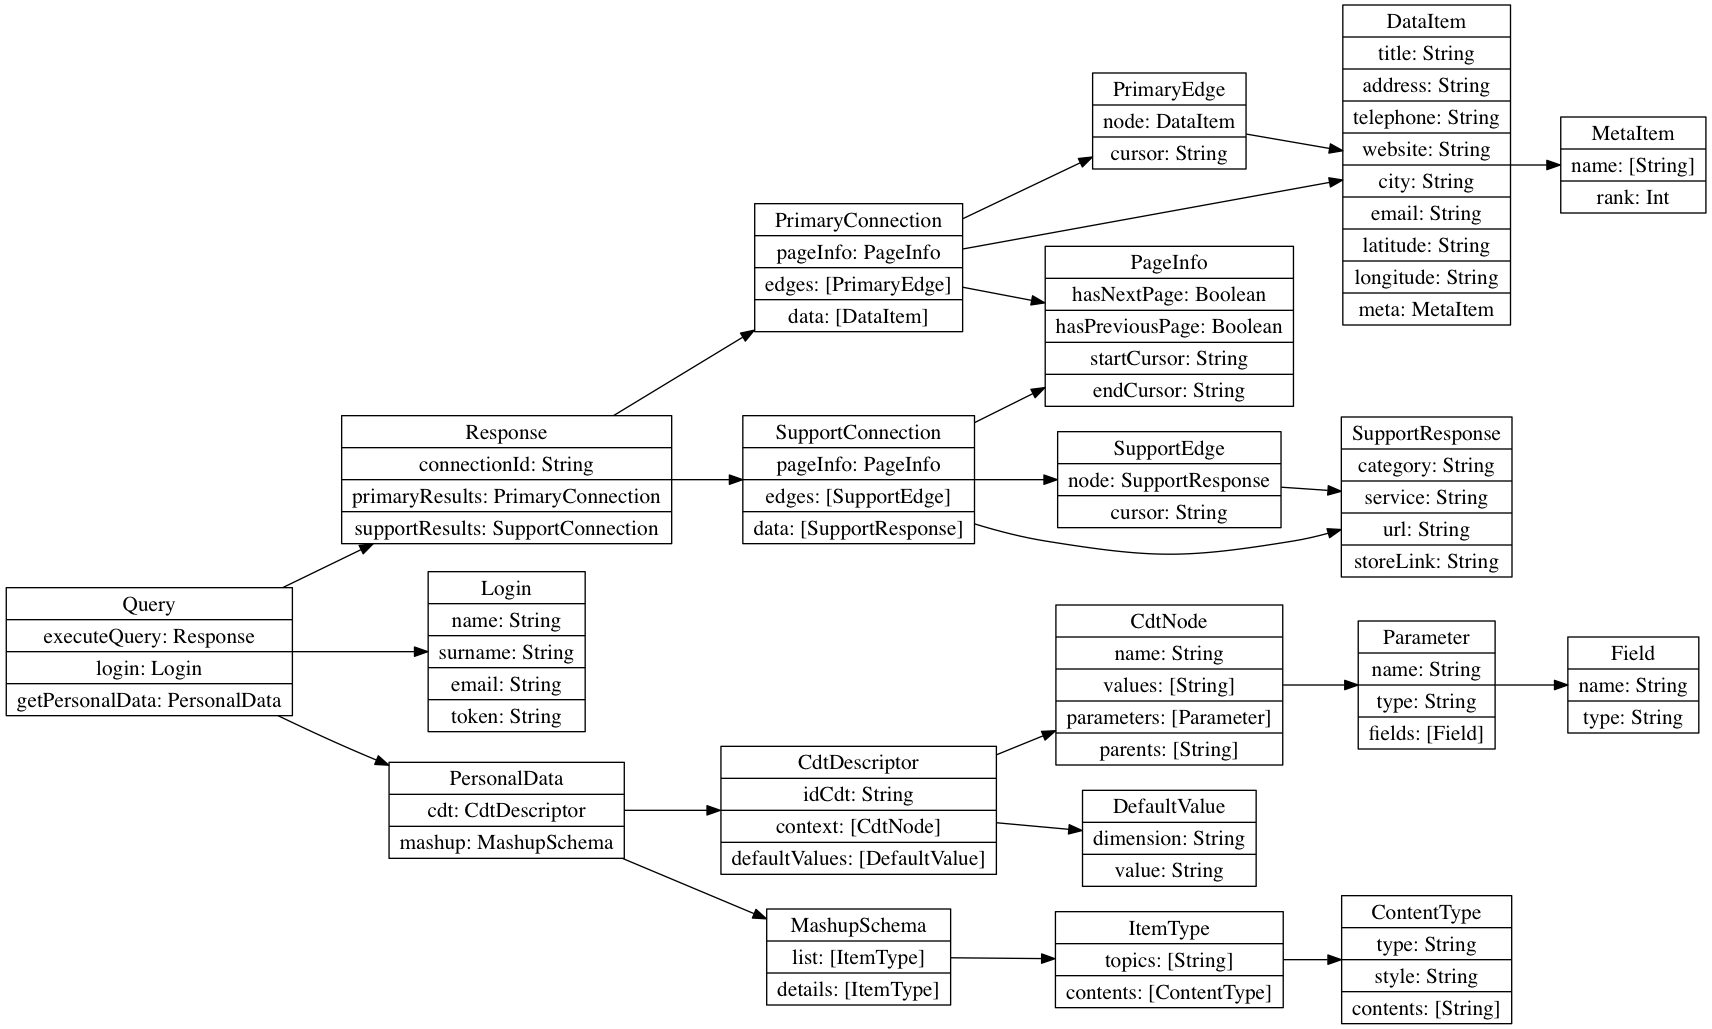
\includegraphics[width=\textwidth]{5-implementazione-backend/Immagini/graphql-schema.png}
	\caption{Diagramma dello schema GraphQL}\label{fig:schema-graphql}
\end{figure}

Il resto di questa sezione descriverà in dettaglio le varie attività che possono essere invocate. Esse saranno identificate per semplicità di espressione col nome \virgolette{endpoint}, visto che il fine ultimo è paragonabile a quello degli \emph{endpoint} nel mondo REST.

\subsection{Execute Query\label{sec:execute-query-endpoint}}

\upe l'\emph{endpoint} principale, riceve in ingresso il contesto dell'utente e restituisce le informazioni recuperate, divise in \emph{primarie} e di \emph{supporto}. L'oggetto accettato in ingresso è composto dai seguenti campi:

\begin{itemize}
	\item \textbf{User Mail}
	L'indirizzo \emph{mail} dell'utente
	\item \textbf{Id Cdt}
	\upe l'identificativo dell'albero di contesto che si desidera utilizzare
	\item \textbf{Context}
	Contiene le informazioni di contesto, ossia i nodi che sono attivi. Ogni oggetto è composto dai seguenti attributi:
	\begin{itemize}
		\item \textbf{Dimension}
		Rappresenta il nome del nodo dimensione
		\item \textbf{Value}
		Contiene il valore selezionato dall'utente per la dimensione
		\item \textbf{Parameters}
		Elenca i parametri associati alla dimensione. Ogni parametro è strutturato come di seguito:
		\begin{itemize}
			\item \textbf{Name}
			Il nome del parametro
			\item \textbf{Value}
			Il valore definito dall'utente
			\item \textbf{Fields}
			Contiene l'elenco dei campi associati al parametro. Ogni campo viene descritto dal proprio \virgolette{nome} e dal \virgolette{valore} che assume
		\end{itemize}
	\end{itemize}
	\item \textbf{Support}
	Contiene l'elenco delle categorie di servizi di supporto che si vogliono ricevere
\end{itemize}

Una volta ricevuto l'oggetto col \emph{contesto}, tramite l'\emph{Execution Helper} viene creato il \emph{CDT Decorato}. Una volta creato, verrà utilizzato come base per l'acquisizione delle informazioni e la composizione dei servizi di supporto. Viene definito il seguente oggetto come risposta:

\begin{itemize}
	\item \textbf{Connection Id}
	Identificativo univoco della sessione. Viene utilizzato per segnalare al \emph{client} se la risposta fa parte di una sessione precedente o si tratta di una nuova sessione
	\item \textbf{Primary Connection}
	Mette a disposizione l'elenco dei risultati integrati forniti dai servizi primari. La particolarità è che si tratta di una \emph{connessione}, una tipologia specifica di \emph{GraphQL} che viene utilizzata quando si ha un elenco di elementi da mostrare. La caratteristica principale che mette a disposizione riguarda la paginazione dei dati. Una volta definita la connessione, sempre tramite l'\emph{Execution Helper}, viene avviato il flusso di richiesta delle informazioni. A \emph{GraphQL} viene restituito un vettore con i risultati. A partire da questo elenco sarà suo compito dividerlo in parti in base alla richiesta ricevuta dal \emph{client}. In particolare vengono utilizzati due parametri per specificare quali elementi si desiderano ricevere: \emph{i)} \emph{first}, dove viene specificato un numero \emph{N} di elementi che si desidera ricevere; \emph{ii)} \emph{after}, che definisce il cursore dell'ultimo elemento ricevuto nella richiesta precedente. Quando viene utilizzato unicamente il campo \virgolette{first}, \emph{GraphQL} restituisce i primi \emph{N} risultati. Se viene specificato anche il campo \virgolette{after} vengono mostrati gli \emph{N} elementi a partire dall'elemento successivo a quello definito dal cursore. Per cursore si intende un identificativo univoco che viene automaticamente calcolato da \emph{GraphQL} per ogni elemento della risposta. Per permettere al \emph{client} di conoscere lo stato della paginazione oltre all'elenco dei risultati viene restituito anche un oggetto di stato, contenente principalmente due attributi: \emph{i)} \emph{hasNextPage}, valore booleano che indica se può essere recuperata un'ulteriore pagina; \emph{ii)} \emph{endCursor}, che fornisce il cursore dell'ultimo elemento ricevuto nella richiesta corrente. In questo modo viene lasciata libertà al \emph{client} di gestire il numero di elementi da ricevere. Ogni oggetto che della risposta è composto dai \emph{termini semantici} che sono stati definiti nel sistema. Inoltre viene aggiunto un oggetto che indica da quali servizi, che possono essere più di uno nel caso di unione di elementi duplicati, è stato recuperato l'oggetto e il punteggio assegnato al servizio in fase di selezione
	\item \textbf{Support Connection}
	Fornisce l'elenco dei servizi di supporto che sono stati selezionati. Come nel caso dei risultati primari viene utilizzata una \emph{connessione} GraphQL. Ogni oggetto viene rappresentato dal \emph{nome} del servizio, la \emph{categoria} per la quale è stato selezionato e l'\emph{indirizzo} composto
\end{itemize}

Nel Listato \ref{lst:esempio-richiesta-execute-query} viene mostrato un esempio di richiesta per effettuare la ricerca di dati sia \emph{primari} sia di \emph{supporto}.

\subsection{Login\label{sec:login-endpoint}}

Questo \emph{endpoint} è dedicato all'autenticazione degli utenti. Riceve in ingresso l'indirizzo \emph{mail} e la \emph{password}, cifrata con algoritmo \emph{SHA1}\footnote{SHA1: \url{https://en.wikipedia.org/wiki/SHA-1}}, digitati dall'utente. Se i due parametri corrispondono a un utente vengono restituiti un \emph{token}, utilizzato per mantenere aperta la sessione, e il \emph{nome} e \emph{cognome} dell'utente, per personalizzare l'\emph{app} con le informazioni personali.

\subsection{Get Personal Data\label{sec:get-personal-data-endpoint}}

Questo \emph{endpoint} provvede a fornire all'utente i suoi dati personali, che possono essere gli \emph{alberi di contesto} e i \emph{mashup} che gli sono stati associati dall'esperto di settore. In questo modo la \emph{mobile app} può recuperare le versioni più aggiornate degli schemi relativi all'utente. In ingresso vengono richiesti l'\emph{indirizzo mail} dell'utente e il \emph{token} ricevuto nella fase di autenticazione. Se i due valori corrispondono, vengono restituiti i dati richiesti. Il formato della risposta viene composto come segue:

\begin{itemize}
	\item \textbf{Cdt}
	Rappresenta la radice dell'albero di contesto. Un \emph{CDT} viene definito dai seguenti attributi:
	\begin{itemize}
		\item \textbf{Id Cdt}
		L'identificativo dell'albero di contesto
		\item \textbf{Context}
		Contiene le informazioni sul contesto, ossia i nodi che compongono l'albero. Ciascun nodo viene definito come segue:
		\begin{itemize}
			\item \textbf{Name}
			Il nome del nodo dimensione
			\item \textbf{Values}
			L'elenco dei possibili valori che può assumere il nodo
			\item \textbf{Parameters}
			Lista dei parametri associati al nodo. Ogni parametro è composto dai seguenti campi:
			\begin{itemize}
				\item \textbf{Name}
				Il nome dell'attributo
				\item \textbf{Type}
				La tipologia di dato
				\item \textbf{Fields}
				Elenco di campi che specializzano il parametro. La struttura di un campo è molto simile a quella del parametro, infatti contiene gli attributi \virgolette{Name}, che definisce il nome del campo, e \virgolette{Type}, che ne specifica la tipologia
			\end{itemize}
			\item \textbf{Parents}
			Elenco di tutti i parenti del nodo corrente
		\end{itemize}
		\item \textbf{Default Values}
		Elenco dei valori che non vengono mostrati nell'albero di contesto perché precedentemente selezionati. Questo oggetto è composto dagli attributi \virgolette{dimension}, che rappresenta il nome del nodo dimensione, e \virgolette{value}, che è il valore associato al nodo
	\end{itemize}
	\item \textbf{Mashup}
	Rappresenta lo schema dei \emph{mashup}. Fornisce alla \emph{mobile app} le regole per comporre l'interfaccia grafica nelle diverse situazioni. Uno schema di \emph{mashup} è composto dai seguenti campi:
	\begin{itemize}
		\item \textbf{List}
		Questo oggetto fornisce le regole per rappresentare la lista dei risultati, ossia la schermata di \emph{merge} o \emph{master}. In questa pagina viene mostrato l'elenco dei dati recuperati, descritti da un insieme ridotto di attributi. Per specificare quali dati devono essere mostrati e come vengono utilizzati i seguenti attributi:
		\begin{itemize}
			\item \textbf{Topics}
			Elenco degli \emph{Interest Topic} per i quali lo schema corrente è valido
			\item \textbf{Contents}
			Definisce i componenti che devono essere utilizzati, il loro stile e dove recuperare i dati da essere mostrati. Ogni oggetto viene definito dai seguenti attributi:
			\begin{itemize}
				\item \textbf{Type}
				Specifica la tipologia di componente da utilizzare (es.: \emph{text} per informazioni testuali, \emph{map} per mostrare una mappa, \emph{website} per creare un collegamento verso una pagina web, ecc.)
				\item \textbf{Style}
				Permette di definire uno stile diverso da quello predefinito al componente. Se è presente permette di sovrascrivere lo stile originale \emph{Flexbox} dell'elemento
				\item \textbf{Contents}
				Definisce quali sono i \emph{termini semantici} dai quali è possibile recuperare le informazioni. Viene inoltre data la possibilità di inserire dei sottocomponenti, dello stesso tipo definito nell'attributo \virgolette{Type}, per formare un componente aggregato
			\end{itemize}
		\end{itemize}	
		\item \textbf{Details}
		Questo oggetto definisce la composizione della schermata di dettaglio di un singolo elemento. Questa pagina viene richiamata una volta che l'utente seleziona un elemento per controllarne le informazioni specifiche. Viene definito dagli stessi attributi della sezione \virgolette{List}			
	\end{itemize}
\end{itemize}

Nel Listato \ref{lst:esempio-get-personal-data} viene mostrato un esempio di richiesta per ricevere i dati personali dell'utente.

\section{File di configurazione\label{sec:file-configurazione}}

Per configurare agilmente determinati parametri del sistema, vengono sfruttate le \emph{variabili d'ambiente} e viene messa a disposizione una cartella dove aggiungere dei \emph{file di configurazione}. In caso di conflitto viene seguita la seguente scala di priorità:

\begin{enumerate}
	\item \textbf{Variabili d'ambiente}
	Vengono inizialmente considerate le variabili d'am\-bien\-te
	\item \textbf{File di configurazione}
	Il valore viene acquisito dal file di configurazione
	\item \textbf{Valore predefinito}
	Se nessuno dei due precedenti passi ha prodotto un valore ne viene utilizzato uno predefinito. Esistono casi dove un valore predefinito non è utilizzabile (es.: indirizzo del database), quindi se non viene specificato alcun valore l'applicazione lancerà un'eccezione
\end{enumerate}

Vengono messe a disposizione le seguenti variabili d'ambiente:

\begin{itemize}
	\item \textbf{NODE\_ENV}
	Per definire l'ambiente nel quale avviare l'applicazione (es.: \emph{production}, \emph{development}, \emph{testing}, ecc.)
	\item \textbf{PORT}
	La porta che si vuole utilizzare per richiamare gli \emph{endpoint}
	\item \textbf{MONGO\_URI}
	L'indirizzo di \emph{MongoDB}. Può comprendere anche l'utente e la \emph{password} di accesso al database
	\item \textbf{REDIS\_URL}
	L'indirizzo di \emph{Redis}. Può comprendere anche l'utente e la \emph{password} di accesso al database
\end{itemize}

Nella cartella \virgolette{config} è possibile aggiungere dei file per configurare altri parametri. Possono essere creati più file di configurazione, che verranno caricati per i diversi ambienti nel quale può funzionare l'applicazione. Basta chiamare il file col nome dell'ambiente di destinazione (es.: \emph{production}, \emph{development}, \emph{qa}, \emph{staging}, ecc.) affinché venga selezionata la configurazione corretta. Viene fornita una configurazione di \virgolette{default}, utilizzata quando non è presente nessun file relativo all'ambiente corrente. Di seguito vengono elencati i parametri che possono essere configurati; tra parentesi sono indicati i valori predefiniti di ciascun campo:

\begin{itemize}
	\item \textbf{server}
	Contiene la configurazione del server
	\begin{itemize}
		\item \textbf{port}
		(3001) Definisce la porta che si vuole utilizzare per richiamare l'\emph{endpoint}
	\end{itemize}
	\item \textbf{database}
	Contiene la configurazione di \emph{MongoDB}
	\begin{itemize}
		\item \textbf{address}
		Definisce l'indirizzo del database. Possono essere incluse le informazioni di autenticazione
	\end{itemize}
	\item \textbf{redis}
	Definisce la configurazione di \emph{Redis}
	\begin{itemize}
		\item \textbf{address}
		(localhost:6379) Specifica l'indirizzo del database \emph{in-memory}. Possono essere incluse le informazioni di autenticazione
	\end{itemize}
	\item \textbf{rest}
	Specifica la configurazione del \emph{bridge} per i servizi REST
	\begin{itemize}
		\item \textbf{timeout}
		Definisce i periodi di tempo dopo i quali scatta il \emph{timeout}
		\begin{itemize}
			\item \textbf{service}
			(3000) Valore di \emph{timeout} dopo il quale una richiesta verso i servizi esterni scade. Il valore viene specificato in millisecondi (ms)
			\item \textbf{cache}
			(1800) Specifica il tempo per il quale rimangono salvati in \emph{cache} le risposte ricevute dai servizi. Il tempo viene espresso in secondi (s)
		\end{itemize}
	\end{itemize}
	\item \textbf{primaryService}
	Gestisce la configurazione del componente \emph{Primary Service Selection}
	\begin{itemize}
		\item \textbf{n}
		(3) Definisce quante operazioni selezionare
		\item \textbf{weight}
		Specifica i pesi che vengono assegnati alle varie tipologie di nodo
		\begin{itemize}
			\item \textbf{filter}
			(1) Peso dei nodi di tipo \emph{filter}
			\item \textbf{ranking}
			(4) Peso dei nodi di tipo \emph{ranking}
		\end{itemize}
	\end{itemize}
	\item \textbf{similarity}
	Configurazione del componente di ricerca dei duplicati
	\begin{itemize}
		\item \textbf{threshold}
		(0.85) Definisce la percentuale minima di similarità tra due elementi affinché vengano considerati duplicati. Una valore maggiore indica un'elevata similarità tra gli elementi. Viene considerato come una percentuale (es.: 0.9 equivale al 90\% di similarità)
	\end{itemize}
	\item \textbf{paginationTTL}
	(1800) Definisce il tempo per il quale rimane memorizzato lo stato di una connessione in \emph{cache}. Il tempo viene specificato in secondi (s)
	\item \textbf{debug}
	(false) Indicatore booleano che abilita o disabilita il \emph{logging} delle informazioni su \emph{console}
	\item \textbf{metrics}
	(false) Valore booleano che abilita o disabilita la raccolta delle informazioni sui tempi di esecuzione dei metodi principali e delle chiamate verso i database
\end{itemize}

Nessun campo è obbligatorio, a eccezione dell'indirizzo di \emph{MongoDB}, se non specificato tramite \emph{variabili d'ambiente}. In assenza degli altri campi verranno utilizzati i rispettivi valori di \emph{default}.